\documentclass[10pt]{beamer}\usepackage[]{graphicx}\usepackage[]{color}
% maxwidth is the original width if it is less than linewidth
% otherwise use linewidth (to make sure the graphics do not exceed the margin)
\makeatletter
\def\maxwidth{ %
  \ifdim\Gin@nat@width>\linewidth
    \linewidth
  \else
    \Gin@nat@width
  \fi
}
\makeatother

\definecolor{fgcolor}{rgb}{0.345, 0.345, 0.345}
\newcommand{\hlnum}[1]{\textcolor[rgb]{0.686,0.059,0.569}{#1}}%
\newcommand{\hlstr}[1]{\textcolor[rgb]{0.192,0.494,0.8}{#1}}%
\newcommand{\hlcom}[1]{\textcolor[rgb]{0.678,0.584,0.686}{\textit{#1}}}%
\newcommand{\hlopt}[1]{\textcolor[rgb]{0,0,0}{#1}}%
\newcommand{\hlstd}[1]{\textcolor[rgb]{0.345,0.345,0.345}{#1}}%
\newcommand{\hlkwa}[1]{\textcolor[rgb]{0.161,0.373,0.58}{\textbf{#1}}}%
\newcommand{\hlkwb}[1]{\textcolor[rgb]{0.69,0.353,0.396}{#1}}%
\newcommand{\hlkwc}[1]{\textcolor[rgb]{0.333,0.667,0.333}{#1}}%
\newcommand{\hlkwd}[1]{\textcolor[rgb]{0.737,0.353,0.396}{\textbf{#1}}}%
\let\hlipl\hlkwb

\usepackage{framed}
\makeatletter
\newenvironment{kframe}{%
 \def\at@end@of@kframe{}%
 \ifinner\ifhmode%
  \def\at@end@of@kframe{\end{minipage}}%
  \begin{minipage}{\columnwidth}%
 \fi\fi%
 \def\FrameCommand##1{\hskip\@totalleftmargin \hskip-\fboxsep
 \colorbox{shadecolor}{##1}\hskip-\fboxsep
     % There is no \\@totalrightmargin, so:
     \hskip-\linewidth \hskip-\@totalleftmargin \hskip\columnwidth}%
 \MakeFramed {\advance\hsize-\width
   \@totalleftmargin\z@ \linewidth\hsize
   \@setminipage}}%
 {\par\unskip\endMakeFramed%
 \at@end@of@kframe}
\makeatother

\definecolor{shadecolor}{rgb}{.97, .97, .97}
\definecolor{messagecolor}{rgb}{0, 0, 0}
\definecolor{warningcolor}{rgb}{1, 0, 1}
\definecolor{errorcolor}{rgb}{1, 0, 0}
\newenvironment{knitrout}{}{} % an empty environment to be redefined in TeX

\usepackage{alltt}


%\input{slides_header.tex}
\input{/home/sahir/git_repositories/epib607/inst/slides/slides_header2.tex}
\graphicspath{{/home/sahir/git_repositories/epib607/inst/slides/figure/}}


\newcommand{\Var}{\operatorname{Var}}
\newcommand{\Expec}{\operatorname{E}}
\newcommand{\Prob}{\operatorname{P}}

%\let\oldShaded\Shaded
%\let\endoldShaded\endShaded
%\renewenvironment{Shaded}{\footnotesize\oldShaded}{\endoldShaded}

%\newcommand{\blue}[1]{\textcolor{blue}{#1}}
%\newcommand{\red}[1]{\textcolor{red}{#1}}


\usepackage{xparse}
\NewDocumentCommand\mylist{>{\SplitList{;}}m}
{
	\begin{itemize}
		\ProcessList{#1}{ \insertitem }
	\end{itemize}
}
\NewDocumentCommand\mynum{>{\SplitList{;}}m}
{
	\begin{enumerate}
		\ProcessList{#1}{ \insertitem }
	\end{enumerate}
}
\newcommand\insertitem[1]{\item #1}

\newcommand\FrameText[1]{%
	\begin{textblock*}{\paperwidth}(0pt,\textheight)
		\raggedright #1\hspace{.5em}
\end{textblock*}}
\IfFileExists{upquote.sty}{\usepackage{upquote}}{}
\begin{document}
	
	
	


	
	\title{024 - Logistic Regression I}
	\author{EPIB 607}
	\institute{
		Sahir Rai Bhatnagar\\
		Department of Epidemiology, Biostatistics, and Occupational Health\\
		McGill University\\
		
		\vspace{0.1 in}
		
		\texttt{sahir.bhatnagar@mcgill.ca}\\
		%\texttt{\url{https://sahirbhatnagar.com/EPIB607/}}
	}
	
	\date{slides compiled on \today}
	
	\maketitle
	
	%\section{Objectives}
	


\section{Logistic Regression}

\begin{frame}{Confounding revisited}

\begin{itemize}
	\item The study on success of different kidney stone removal procedures reported by Charig et al. (1986) provides a nice and clean example of confounding, where the direction of the estimated effect size is reversed by introducing stratification.
\item The procedure, either open surgery, percutaneous nephrolithotomy (PN, a keyhole surgery procedure) or extracorporeal shock wave lithotripsy (ESWL), was defined to be successful if stones were eliminated or reduced to less than $2 \mathrm{~mm}$ after three months.
\item The study collected cases of kidney stones treated at a particular UK hospital during $1972-1985$.
\item 350 of these cases were treated with open surgery and 350 with percutaneous nephrolithotomy.
\end{itemize}
\end{frame}


\begin{frame}{Outcome data}
\begin{itemize}
	\item The counts of successes for the two surgical procedures were:
	$$
	\begin{array}{lccc}
	                       &\texttt{Unsuccessful}& \texttt{Successful}& \texttt{Total}\\
	\text { Open surgery } & 77 & 273 & 350 \\
	\text { PN } & 61 & 289 & 350 \\
	\text { Total } & 138 & 562 & 700
	\end{array}
	$$
	\item  Empirical odds ratio for the failure of the procedure is given by
	$$
	\log \left(\frac{77 / 273}{61 / 289}\right)=\log \left(\frac{77 \times 289}{61 \times 273}\right) \approx 0.290
	$$
	and its standard error by
	$$
	\sqrt{\frac{1}{77}+\frac{1}{61}+\frac{1}{273}+\frac{1}{289}} \approx 0.191
	$$
	\item Open surgery appears to have higher odds of failure, although the log-odds ratio estimate is smaller than two times the standard error.
\end{itemize}
\end{frame}


\begin{frame}{Interpretation}
\begin{itemize}
	\item Based on these results, do we have evidence that percutaneous nephrolithotomy is more effective than open surgery?
	\item It certainly is less invasive.
	\item Similar pattern can be observed for instance for kidney (and other) cancer surgeries; the patients treated with the less invasive procedure have better outcomes, at least in the short term.
	\item  What is really going on here?
	\item  Remember that the treatment procedure was not randomized; the cases were ascertained from the hospital records.
	\item  Recall 'the triangle'.
\end{itemize}
\end{frame}


\begin{frame}{The triangle}
\centering
\includegraphics[width=\linewidth]{triangle.png}
\vspace{0.3in}
$\text { What are } X, Y \text { and } Z \text { in the present example? }$
\end{frame}


\begin{frame}{Outcomes by kidney stone size}
	\begin{itemize}
		\item Below are the same outcomes tabulated by the size of the kidney stone (smaller than $2 \mathrm{~cm} /$ at least $2 \mathrm{~cm}$ in diameter $)$
		
		\vspace{0.2in}
		
		
$\begin{array}{lccc}
	<2 \mathrm{~cm} & \text { Unsuccessful } & \text { Successful } & \text { Total } \\
	\text { Open surgery } & 6 & 81 & 87 \\
	\text { PN } & 36 & 234 & 270 \\
	\text { Total } & 42 & 315 & 357 \\
	& & & \\
	\geq 2 \mathrm{~cm} & \text { Unsuccessful } & \text { Successful } & \text { Total } \\
	\text { Open surgery } & 71 & 192 & 263 \\
	\text { PN } & 25 & 55 & 80 \\
	\text { Total } & 96 & 247 & 343
\end{array}$
	\end{itemize}
\end{frame}


\begin{frame}{Stratum-specific odds ratios}
	\begin{itemize}
		\item The empirical odds ratio and its standard error in the $<2$
		cm group are
		$$
		\log \left(\frac{6 \times 234}{36 \times 81}\right) \approx-0.731
		$$
		and
		$$
		\sqrt{\frac{1}{6}+\frac{1}{36}+\frac{1}{81}+\frac{1}{234}} \approx 0.459
		$$
		\item Similarly, these numbers in the $\geq 2 \mathrm{~cm}$ group are
		$$
		\log \left(\frac{71 \times 55}{25 \times 192}\right) \approx-0.206
		$$
		and
		$$
		\sqrt{\frac{1}{71}+\frac{1}{25}+\frac{1}{192}+\frac{1}{55}} \approx 0.278
		$$
		\item Now open surgery appears to have lower odds of failure within the strata.
	\end{itemize}
	
\end{frame}


\begin{frame}{Interpretation}
\begin{itemize}
	\item Open surgery was much more common in the $\geq 2 \mathrm{~cm}$ group, as was the failure of surgery.
	\item  This is not surprising; presumably larger stones are more difficult to remove, whilst also requiring a more invasive procedure.
	\item  Prima facie this seems to be an example of confounding by indication, with kidney stone size being part of the indication for the choice between open and keyhole
	surgery.
	\item  Was kidney stone size known before the choice of the procedure, or was the indication related to something else, perhaps symptomatic of the size?
	\item  How exactly were the cases selected?
\end{itemize}
\end{frame}




\begin{frame}{Stratified analysis}
	\begin{itemize}
		\item It is obvious that the first pooled analysis was confounded.
		\item  Within stratum estimates are more valid.
		\item  How can we combine the results across strata without
		re-introducing the confounding?
		\item  We have to take a weighted average of the stratum-specific log-odds ratios.
		\item  Let now $\log \hat{\theta}_{0}$ and $\log \hat{\theta}_{1}$ be the empirical log-odds ratios within the $<2 \mathrm{~cm}$ and $\geq 2 \mathrm{~cm}$ groups, respectively.
		\item  Weighted average of these is given by
		$$
		\log \hat{\theta}=\frac{w_{0} \log \hat{\theta}_{0}+w_{1} \log \hat{\theta}_{1}}{w_{0}+w_{1}}=\frac{\sum_{j=0}^{1} w_{j} \log \hat{\theta}_{j}}{\sum_{j=0}^{1} w_{j}}
		$$
		\item  How to choose the weights?
	\end{itemize}
\end{frame}



\begin{frame}{The Woolf 1955 method}
	\begin{itemize}
		\item Presumably the choice of the weights must depend on the stratum sizes since a large stratum would be more informative than a small one, requiring larger weight in the combined estimate. 
		\item In fact, the quantity $\frac{1}{S^{2}}$ is known as the observed information.
		\item Accordingly, in the Woolf 1955 method for stratified analysis, the weights are chosen as
		$$
		w_{j}=\frac{1}{\frac{1}{D_{1 j}}+\frac{1}{D_{0 j}}+\frac{1}{H_{1 j}}+\frac{1}{H_{0 j}}}
		$$
		\item Now we have
		$$
		w_{0}=\frac{1}{\frac{1}{6}+\frac{1}{36}+\frac{1}{81}+\frac{1}{234}} \approx 4.738
		$$
		and
		$$
		w_{1}=\frac{1}{\frac{1}{71}+\frac{1}{25}+\frac{1}{192}+\frac{1}{55}} \approx 12.907
		$$
	\end{itemize}
\end{frame}




\begin{frame}{Combined estimate and its standard error}
	\begin{itemize}
		\item With these weights, the combined estimate is given by
		$$
		\log \hat{\theta}=\frac{4.738 \times-0.731+12.907 \times-0.206}{4.738+12.907} \approx-0.347
		$$
		\item Standard error is the square root of the inverse of the total information.
		\item  Information is additive.
		\item  Thus, the standard error of the combined estimate is given by
		$$
		\sqrt{\frac{1}{\frac{1}{S_{0}^{2}}+\frac{1}{S_{1}^{2}}}}=\sqrt{\frac{1}{w_{0}+w_{1}}}=\sqrt{\frac{1}{4.738+12.907}} \approx 0.238
		$$
	\end{itemize}
\end{frame}



\begin{frame}{Limitations of stratified analysis}
	\begin{itemize}
		\item In the similar Mantel-Haenszel method, the stratum-specific weights are given by $w_{j}=\frac{H_{1 j} D_{0 j}}{N_{j}},$ where $N_{j}$ is the total $N$ of table $j$
		\item  The Woolf and Mantel-Haenszel methods are applicable only when there are no zero cell counts in any of the confounder-conditional $2 \times 2$ -tables.
		\item  This becomes an issue whenever there are a large number of confounder strata.
		\item  Usually one would have a large number of potential confounders, some of which are continuous-valued, so cross-stratifying across all of these quickly becomes infeasible.
		\item  The problem needs to be re-parametrized in more parsimonious way.
	\end{itemize}
\end{frame}

\begin{frame}{Another example}
	\begin{itemize}
		\item Senn (2003) used these diabetes cohort data to
		demonstrate \textit{Simpson's paradox}:
		
		$$
		\begin{array}{lccc} 
			& \text { Dead } & \text { Censored } & \text { Total } \\
			\text { Type II } & 218 & 326 & 544 \\
			\text { Type I } & 105 & 253 & 323 \\
			\text { Total } & 323 & 579 & 902
		\end{array}
		$$
		
		\item Empirical all-cause mortality odds ratio is given by
		$$
		\log \left(\frac{218 \times 253}{105 \times 326}\right) \approx 0.477
		$$
		and its standard error by
		$$
		\sqrt{\frac{1}{218}+\frac{1}{105}+\frac{1}{326}+\frac{1}{253}} \approx 0.145
		$$
		\item Type II diabetes patients seem to have higher mortality.
	
	
	\end{itemize}
\end{frame}



\begin{frame}{Mortality outcomes by age group}
	\begin{itemize}
		\item Below are the same outcomes tabulated by age:
		
		$$
		\begin{array}{lccc}
		\leq 40 & \text { Dead } & \text { Censored } & \text { Total } \\
		\text { Type II } & 0 & 15 & 15 \\
		\text { Type I } & 1 & 129 & 130 \\
		\text { Total } & 1 & 144 & 145 \\
		& & & \\
		& & & \\
		>40 & \text { Dead } & \text { Censored } & \text { Total } \\
		\text { Type II } & 218 & 311 & 529 \\
		\text { Type I } & 104 & 124 & 228 \\
		\text { Total } & 322 & 435 & 757
		\end{array}
		$$
		\item There is only one death and very few type II diabetes patients in the $\leq 40$ age group.
		\item Obviously, age is a determinant of both the type of diabetes and mortality.
	\end{itemize}
\end{frame}



\begin{frame}{Stratum-specific log-odds ratios}
	\begin{itemize}
		\item The empirical log-odds ratio and its standard error in the $\leq 40$ group are
		$$
		\log \left(\frac{0 \times 129}{1 \times 15}\right)=-\infty
		$$
		and
		$$
		\sqrt{\frac{1}{0}+\frac{1}{1}+\frac{1}{15}+\frac{1}{129}}=\text { undefined }
		$$
		\item  These numbers in the $>40$ group are
		$$
		\log \left(\frac{218 \times 124}{104 \times 311}\right) \approx-0.179
		$$
		and
		$$
		\sqrt{\frac{1}{71}+\frac{1}{25}+\frac{1}{192}+\frac{1}{55}} \approx 0.160
		$$
		\item Type II diabetes patients over 40 years of age seem to have lower mortality (although not significantly so).
	\end{itemize}
\end{frame}



\begin{frame}{Interpretation}
	\begin{itemize}
		\item Now stratified analysis is not feasible; the $\leq 40$ table is not informative of the mortality log-odds ratio.
		\item Given the row totals, the observed data comprise four death counts, with the numbers of censored given by the row total minus death count.
		\item From four observations, we can estimate at most four
		parameters; the stratum-specific odds ratios both involve two odds parameters.
		\item However, now one of the observed counts is zero, so we are reduced to estimating only three parameters.
		\item The problem needs to be re-parametrized in a more parsimonious way.
	\end{itemize}
\end{frame}



\begin{frame}{Parametrization in terms of risk}
	\begin{itemize}
		\item Introduce a variable $X$ to denote the age group, with $X=0$ for the $\leq 40$ group and $X=1$ for the $>40$ group.
		\item Now we have four risk parameters $\pi_{Z X},$ one for each level of $Z$ and $X:$
		
		$$
		\begin{array}{llcc} 
			     &      & \text { Dead } & \text { Censored } \\
			X=0: & Z=1 & \pi_{10} & 1-\pi_{10} \\
			     & Z=0 & \pi_{00} & 1-\pi_{00} \\
			        & & & \\
			     &  & \text { Dead } & \text { Censored } \\
			X=1:& & \pi_{11}      & 1-\pi_{11} \\
			 & & \pi_{01} & 1-\pi_{01}
		\end{array}
		$$
		\item Risk parameter is a probability, taking values in the $[0, 1]$-interval.
	\end{itemize}
\end{frame}



\begin{frame}{Parametrization in terms of odds}
	\begin{itemize}
		\item Alternatively, we may opt to parametrize in terms of odds,
		that is, risk divided by one minus itself:
		
				$$
		\begin{array}{llcc} 
		&      & \text { Dead } & \text { Censored } \\
		X=0: & Z=1 & \frac{\pi_{10}}{1-\pi_{10}} & \frac{1-\pi_{10}}{\pi_{10}} \\
		& Z=0 & \frac{\pi_{00}}{1- \pi_{00}} & \frac{1-\pi_{00}}{\pi_{00}} \\
		& & & \\
		&  & \text { Dead } & \text { Censored } \\
		X=1:&  Z=1 & \frac{\pi_{11}}{1-\pi_{11}}      & \frac{1-\pi_{11}}{\pi_{11}} \\
		    &  Z=0    & \frac{\pi_{01}}{1-\pi_{01}} & \frac{1-\pi_{01}}{\pi_{01}}
		\end{array}
		$$
		
		\item An odds parameter may take values in the $[0, \infty]$-interval.
	\end{itemize}
\end{frame}




\begin{frame}{Parametrization in terms of log odds}
	\begin{itemize}
		\item Or we may prefer log-odds:
		
		$$
		\begin{array}{llcc} 
		&      & \text { Dead } & \text { Censored } \\
		X=0: & Z=1 & \log\frac{\pi_{10}}{1-\pi_{10}} & \log\frac{1-\pi_{10}}{\pi_{10}} \\
		& Z=0 & \log\frac{\pi_{00}}{1- \pi_{00}} & \log\frac{1-\pi_{00}}{\pi_{00}} \\
		& & & \\
		&  & \text { Dead } & \text { Censored } \\
		X=1:&  Z=1 & \log\frac{\pi_{11}}{1-\pi_{11}}      & \log\frac{1-\pi_{11}}{\pi_{11}} \\
		&  Z=0    & \log\frac{\pi_{01}}{1-\pi_{01}} & \log\frac{1-\pi_{01}}{\pi_{01}}
		\end{array}
		$$
		
		\item A log-odds parameter may take values in the $[-\infty, \infty]$-interval.
		\item Whichever way, there are still four parameters.
		\item How to reduce the number of parameters?
	\end{itemize}
\end{frame}


\begin{frame}{Regression}
	\begin{itemize}
		\item Clayton \& Hills (1993, p. 217)
		\begin{quote}
			A common theme in all these situations is change
			from the original parameters to new parameters
			which are more relevant to the comparisons of
			interest. This change can be described by the
			equations which express the old parameters in
			terms of the new parameters. These equations
			are referred to as \textbf{regression} equations, and the
			statistical model is called a \textbf{regression model}.
		\end{quote}
	
	\item Now the old parameters are the four log-odds:
	
	$$
	\log \frac{\pi_{ZX}}{1-\pi_{ZX}}
	$$
	
	\end{itemize}
\end{frame}





\begin{frame}{Regression equation}
	\begin{itemize}
		\item Reparametrizing the log-odds is referred to as logistic regression.
		\item In the ongoing example we may take
		$$
		\log \left(\frac{\pi_{Z X}}{1-\pi_{Z X}}\right)=\alpha+\beta Z+\gamma X
		$$
		\item The original four parameters are now expressed in terms of three new parameters: an intercept term $\alpha$ and regression coefficients $\beta$ and $\gamma$.
		\item The function $\log \frac{\pi}{1-\pi}$ is referred to as the logit transformation of the risk parameter $\pi$.
		\item Thus, the same model can be specified as a reparametrization of the risk parameter together with the \textit{logit link} function:
		$$
		\operatorname{logit}\left(\pi_{Z X}\right)=\alpha+\beta Z+\gamma X
		$$
	\end{itemize}
\end{frame}





\begin{frame}{Parametrization in terms of regression parameters}
	\begin{itemize}
		\item Through the previous model specification we get the
		log-odds tables
		
				$$
		\begin{array}{llc|c} 
		&      & \text { Dead } & \text { Censored } \\
		X=0: & Z=1 & \textcolor{white}{tfdsfdsftfsafsafasfas} & \textcolor{white}{tfdsfdsftfsafsafasfas} \\
		\hline
		& Z=0 &  &  \\
		& & & \\
		&  & \text { Dead } & \text { Censored } \\
		X=1:&  Z=1 &  &  \\
				\hline
		&  Z=0    &  & 
		\end{array}
		$$
		
		\item How to interpret the new parameters?
		\item Suppose that we are interested in the mortality odds ratio for type II vs. type I diabetes patients, controlling for age.
		\item In other words, our parameter of interest is
		
		$$
		\frac{\frac{\pi_{1X}}{1-\pi_{1X}}}{\frac{\pi_{0X}}{1-\pi_{0X}}}
		$$
		
				
	\end{itemize}
\end{frame}







\begin{frame}{Interpretation of the regression coefficient}
	\begin{itemize}
		\item Through the regression equation we get
		$$
		\begin{aligned}
		\frac{\frac{\pi_{1 X}}{1-\pi_{1 X}}}{\frac{\pi_{0 X}}{1-\pi_{0 X}}} &=\frac{e^{\alpha+\beta+\gamma X}}{e^{\alpha+\gamma X}} \\
		&=\frac{e^{\alpha} e^{\beta} e^{\gamma X}}{e^{\alpha} e^{\gamma X}} \\
		&=e^{\beta} \\
		\Leftrightarrow \log \left(\frac{\frac{\pi_{1 X}}{1-\pi_{1 X}}}{\frac{\pi_{0 X}}{1-\pi_{0 X}}}\right) &=\beta
		\end{aligned}
		$$
		\item The regression coefficient $\beta$ is a log-odds ratio.
		\item Exponentiating it gives the odds ratio of interest.
		\item Having understood regression as a transformation of the original parameters, where and when does the observed outcome data come into play?
	\end{itemize}
\end{frame}





\begin{frame}[fragile]{Observed data}
	\begin{itemize}
		\item The observed data are the four death counts:
		$$
		\begin{array}{llccc} 
		&      & \text { Dead } & \text { Censored } & \text{ Total }\\
		X=0: & Z=1 & D_{10} & N_{10}-D_{10} & N_{10}\\
		& Z=0 & D_{00} & N_{00}-D_{00} & N_{00}\\
		& & & \\
		&  & \text { Dead } & \text { Censored } \\
		X=1:&  Z=1 & D_{11} & N_{11}-D_{11} & N_{11}\\
		&  Z=0    & D_{01} & N_{01}-D_{01} & N_{01}\\
		\end{array}
		$$
		\item These data entered into \texttt{R} are:
\begin{knitrout}\small
\definecolor{shadecolor}{rgb}{0.969, 0.969, 0.969}\color{fgcolor}\begin{kframe}
\begin{alltt}
\hlstd{dead} \hlkwb{<-} \hlkwd{c}\hlstd{(}\hlnum{0}\hlstd{,}\hlnum{1}\hlstd{,}\hlnum{218}\hlstd{,}\hlnum{104}\hlstd{)}
\hlstd{censored} \hlkwb{<-} \hlkwd{c}\hlstd{(}\hlnum{15}\hlstd{,}\hlnum{129}\hlstd{,}\hlnum{311}\hlstd{,}\hlnum{124}\hlstd{)}
\hlstd{z} \hlkwb{<-} \hlkwd{c}\hlstd{(}\hlnum{1}\hlstd{,}\hlnum{0}\hlstd{,}\hlnum{1}\hlstd{,}\hlnum{0}\hlstd{); x} \hlkwb{<-} \hlkwd{c}\hlstd{(}\hlnum{0}\hlstd{,}\hlnum{0}\hlstd{,}\hlnum{1}\hlstd{,}\hlnum{1}\hlstd{)}
\hlkwd{cbind}\hlstd{(dead,censored,z,x)}
\end{alltt}
\begin{verbatim}
##      dead censored z x
## [1,]    0       15 1 0
## [2,]    1      129 0 0
## [3,]  218      311 1 1
## [4,]  104      124 0 1
\end{verbatim}
\end{kframe}
\end{knitrout}
	
	\end{itemize}
\end{frame}




\begin{frame}{Deterministic and stochastic model components}
	\begin{itemize}
		\item 
		The regression equation specifies the deterministic part of the model.
		
		\item This is defined in terms of parameters, conditional on the values of $Z$ and $X$.
		
		\item To complete the model specification, we need to specify the stochastic component of the model, a statistical distribution for the outcome $D_{Z X}$. 
		\item It is already obvious that the appropriate distribution is
		$$
		D_{Z X} \sim \operatorname{Binomial}\left(N_{Z X}, \pi_{Z X}\right)
		$$
		\item Here the risk $\pi_{Z X}$ is given by the regression equation as (verify)
		$$
		\pi_{Z X}=\frac{e^{\alpha+\beta Z+\gamma X}}{1+e^{\alpha+\beta Z+\gamma X}}=\frac{1}{1+e^{-(\alpha+\beta Z+\gamma X)}}
		$$
		\item This inverse transformation is the so-called \textit{expit} function:
		$$
		\pi_{Z X}=\operatorname{logit}^{-1}(\alpha+\beta Z+\gamma X)=\operatorname{expit}(\alpha+\beta Z+\gamma X)
		$$
	\end{itemize}
\end{frame}



\begin{frame}[fragile]{Fitting the model}
\begin{itemize}
	\item We have now specified the model; next we need to fit it to the data, in order to obtain the estimates $\hat{\alpha}$,$\hat{\beta}$,$\hat{\gamma}$ and	their standard errors.
	\item In \texttt{R}, logistic regression models are fitted using the \texttt{glm} function, as
\begin{knitrout}
\definecolor{shadecolor}{rgb}{0.969, 0.969, 0.969}\color{fgcolor}\begin{kframe}
\begin{alltt}
\hlstd{model} \hlkwb{<-} \hlkwd{glm}\hlstd{(}\hlkwd{cbind}\hlstd{(dead,censored)} \hlopt{~} \hlstd{z} \hlopt{+} \hlstd{x,}
               \hlkwc{family}\hlstd{=}\hlkwd{binomial}\hlstd{(}\hlkwc{link}\hlstd{=}\hlstr{"logit"}\hlstd{))}
\end{alltt}
\end{kframe}
\end{knitrout}
	\item Here the outcome data were entered as frequency records.
	\item Alternatively, we could have entered the data as individual level records; the results would be equivalent (verify).
\end{itemize}
\end{frame}




\begin{frame}[fragile]{Results}
\begin{knitrout}
\definecolor{shadecolor}{rgb}{0.969, 0.969, 0.969}\color{fgcolor}\begin{kframe}
\begin{alltt}
\hlstd{model} \hlkwb{<-} \hlkwd{glm}\hlstd{(}\hlkwd{cbind}\hlstd{(dead,censored)} \hlopt{~} \hlstd{z} \hlopt{+} \hlstd{x,}
              \hlkwc{family}\hlstd{=}\hlkwd{binomial}\hlstd{(}\hlkwc{link}\hlstd{=}\hlstr{"logit"}\hlstd{))}
\hlkwd{print}\hlstd{(}\hlkwd{summary}\hlstd{(model),} \hlkwc{signif.stars} \hlstd{=} \hlnum{FALSE}\hlstd{)}
\end{alltt}
\begin{verbatim}
## 
## Coefficients:
##             Estimate Std. Error z value Pr(>|z|)
## (Intercept)  -4.9525     1.0036  -4.935 8.02e-07
## z            -0.1816     0.1595  -1.139    0.255
## x             4.7781     1.0108   4.727 2.28e-06
## 
## (Dispersion parameter for binomial family taken to be 1)
## 
##     Null deviance: 133.81237  on 3  degrees of freedom
## Residual deviance:   0.18471  on 1  degrees of freedom
## AIC: 20.745
## 
## Number of Fisher Scoring iterations: 5
\end{verbatim}
\end{kframe}
\end{knitrout}
\end{frame}



\begin{frame}[fragile]{Confidence interval for the odds ratio}
	\begin{itemize}
		\item As usual, we can transform a $95 \%$ confidence interval on the log-odds ratio scale to the odds ratio scale as
		$$
		\begin{array}{l}
		e^{-0.1816 \pm 1.96 \times 0.1595} \\
		=0.834 \times e^{\pm 0.313} \\
		=(0.610,1.140)
		\end{array}
		$$
		\item The null value is included in the interval.
		\item After adjusting for age, these data do not give evidence against the null
		$$
		\frac{\frac{\pi_{1 X}}{1-\pi_{1 X}}}{\frac{\pi_{0 X}}{1-\pi_{0 X}}}=1
		$$
	\end{itemize}
\end{frame}



\section{Log-linear model for risk}

\begin{frame}[fragile]{Log-linear model for risk}
	\begin{itemize}
		\item Is there some particular reason why we \textit{have} to use the logit link when modeling risk?
		\item Why could we not just parametrize the log-risk as
		$$
		\log(\pi_{ZX}) = \alpha + \beta Z + \gamma X ?
		$$
		\pause 
		\item We can; in this case the regression coefficient $\beta$ would be interpreted as a log-risk ratio:
$$\begin{aligned}
	\frac{\pi_{1 X}}{\pi_{0 X}} &=\frac{e^{\alpha+\beta+\gamma X}}{e^{\alpha+\gamma X}} \\
	&=\frac{e^{\alpha} e^{\beta} e^{\gamma X}}{e^{\alpha} e^{\gamma X}} \\
	&=e^{\beta} \\
	\Leftrightarrow \log \left(\frac{\pi_{1 X}}{\pi_{0 X}}\right) &=\beta
\end{aligned}$$
	\end{itemize}
\end{frame}




\begin{frame}[fragile]{Fitting the log-linear model}
\begin{itemize}
	\item To fit this model, we only need to change the link
	function:
\begin{knitrout}
\definecolor{shadecolor}{rgb}{0.969, 0.969, 0.969}\color{fgcolor}\begin{kframe}
\begin{alltt}
        \hlstd{model} \hlkwb{<-} \hlkwd{glm}\hlstd{(}\hlkwd{cbind}\hlstd{(dead,censored)} \hlopt{~} \hlstd{z} \hlopt{+} \hlstd{x,}
                     \hlkwc{family}\hlstd{=}\hlkwd{binomial}\hlstd{(}\hlkwc{link}\hlstd{=}\hlstr{"log"}\hlstd{))}
\end{alltt}
\end{kframe}
\end{knitrout}
	\item Using the parameter estimates $\hat{\alpha}$, $\hat{\beta}$, and $\hat{\gamma}$, risk estimates could then be obtained through the back-transformation
	$$
	\hat{\pi}_{ZX} = e^{\hat{\alpha} + \hat{\beta} Z + \hat{\gamma} X}
	$$
	\item However, note that there is nothing here bounding the risk
	to values below one.
	\item The log-linear model does bound the risk to non-negative
	values, so as long as the risk is small, log-linear and
	logistic regression models give similar results.
\end{itemize}
\end{frame}

\begin{frame}[fragile]{Results}
\begin{knitrout}
\definecolor{shadecolor}{rgb}{0.969, 0.969, 0.969}\color{fgcolor}\begin{kframe}
\begin{alltt}
\hlstd{model} \hlkwb{<-} \hlkwd{glm}\hlstd{(}\hlkwd{cbind}\hlstd{(dead,censored)} \hlopt{~} \hlstd{z} \hlopt{+} \hlstd{x,}
             \hlkwc{family}\hlstd{=}\hlkwd{binomial}\hlstd{(}\hlkwc{link}\hlstd{=}\hlstr{"log"}\hlstd{))}
\hlkwd{print}\hlstd{(}\hlkwd{summary}\hlstd{(model),} \hlkwc{signif.stars} \hlstd{=} \hlnum{FALSE}\hlstd{)}
\end{alltt}
\begin{verbatim}
## 
## Coefficients:
##             Estimate Std. Error z value Pr(>|z|)
## (Intercept) -4.96656    0.99655  -4.984 6.24e-07
## z           -0.10229    0.08898  -1.150     0.25
## x            4.18210    0.99867   4.188 2.82e-05
## 
## (Dispersion parameter for binomial family taken to be 1)
## 
##     Null deviance: 133.81237  on 3  degrees of freedom
## Residual deviance:   0.19892  on 1  degrees of freedom
## AIC: 20.759
## 
## Number of Fisher Scoring iterations: 5
\end{verbatim}
\end{kframe}
\end{knitrout}
\end{frame}



\begin{frame}[fragile]{Interpretation}
	\begin{itemize}
		\item The results from the log-linear model differ somewhat from the logistic model.
		\item This is unsurprising since the risk in the present example is not small, so we cannot approximate risk ratios by odds ratios.
		\item A $95 \%$ confidence interval for the risk ratio would be
		calculated in the usual way as
		$$
		\begin{array}{l}
		e^{-0.10229 \pm 1.96 \times 0.08898} \\
		=0.903 \times e^{\pm 0.174} \\
		=(0.759,1.075)
		\end{array}
		$$
	\end{itemize}
\end{frame}




\section{Kidney stone removal procedures 1}


\begin{frame}[fragile,plain]
\vspace{-.91in}
	\tiny
The 1986 BMJ article \textit{Comparison of treatment of renal calculi by open surgery, percutaneous nephrolithotomy, and extracorporeal shockwave lithotripsy} by Charig et. al, was a study designed to compare different methods of treating kidney stones in order to establish which was the most cost effective and successful. The procedure, either open surgery, or percutaneous nephrolithotomy (PN, a keyhole surgery procedure), was defined to be successful if stones were eliminated or reduced to less than 2 mm after three months. The study collected cases of kidney stones treated at a particular UK hospital during 1972-1985. The counts of successes for the two surgical procedures were:
\vspace{-.11in}
\begin{table}[h]
	\centering
	\begin{tabular}{lcc|c}
		& Unsuccessful &  Successful & Total\\
		Open surgery & 77 & 273 & 350 \\
		PN & 61 & 289 & 350 \\
		\hline
		Total & 138 & 562 & 700
	\end{tabular}
\end{table}
\vspace{-.21in}
\begin{knitrout}\tiny
\definecolor{shadecolor}{rgb}{0.969, 0.969, 0.969}\color{fgcolor}\begin{kframe}
\begin{verbatim}
## 
## Coefficients:
##             Estimate Std. Error z value Pr(>|z|)
## (Intercept)  -1.5556     0.1409 -11.040   <2e-16
## open          0.2899     0.1911   1.517    0.129
## 
## (Dispersion parameter for binomial family taken to be 1)
## 
##     Null deviance: 2.3148e+00  on 1  degrees of freedom
## Residual deviance: 3.4195e-14  on 0  degrees of freedom
## AIC: 15.696
## 
## Number of Fisher Scoring iterations: 3
\end{verbatim}
\end{kframe}
\end{knitrout}

\end{frame}

\begin{frame}[fragile,plain]
	\vspace*{-5.0in}
	\textbf{1. Mean depth of the ocean (continued)\footnotetext[1]{\tiny{this page is intentionally left blank}}}
	
\end{frame}


\section{Kidney stone removal procedures 2}

\begin{frame}[fragile,plain]
\vspace{-.91in}
\tiny
Below are the same outcomes tabulated by the size of the kidney stone (smaller than 2cm/at least 2cm in diameter):

\begin{table}[h]
	\centering
	\begin{tabular}{lcc|c}
		$<$ 2cm & Unsuccessful &  Successful & Total\\
		Open surgery & 6 & 81 & 87 \\
		PN 			 & 36 & 234 & 270 \\
		\hline
		Total 	& 42 & 315 & 357 \\
		& & &  \\
		$\geq$ 2cm & Unsuccessful &  Successful & Total\\
		Open surgery & 71 & 192 & 263 \\
		PN 			 & 25 & 55 & 80 \\
		\hline
		Total 		& 96 & 247 & 343
	\end{tabular}
\end{table}

\vspace{-.21in}
\begin{knitrout}\tiny
\definecolor{shadecolor}{rgb}{0.969, 0.969, 0.969}\color{fgcolor}\begin{kframe}
\begin{verbatim}
## 
## Coefficients:
##             Estimate Std. Error z value Pr(>|z|)
## (Intercept)  -1.9366     0.1704 -11.361  < 2e-16
## open         -0.3572     0.2291  -1.559    0.119
## size          1.2606     0.2390   5.274 1.33e-07
## 
## (Dispersion parameter for binomial family taken to be 1)
## 
##     Null deviance: 33.1239  on 3  degrees of freedom
## Residual deviance:  1.0082  on 1  degrees of freedom
## AIC: 26.355
## 
## Number of Fisher Scoring iterations: 3
\end{verbatim}
\end{kframe}
\end{knitrout}
\end{frame}

\begin{frame}[fragile,plain]
	\vspace*{-5.0in}
	\textbf{1. Mean depth of the ocean (continued)\footnotetext[1]{\tiny{this page is intentionally left blank}}}
	
\end{frame}

\section{Diabetes cohort data 1}

\begin{frame}[fragile,plain]
	\vspace{-1.31in}
	\tiny
\begin{table}[h]
	\centering
	\begin{tabular}{lcc|c}
		& Dead &  Censored & Total\\
		Type II & 218 & 326 & 544 \\
		Type I & 105 & 253 & 323 \\
		\hline
		Total & 323 & 579 & 902
	\end{tabular}
\end{table}

	\vspace{-.21in}
\begin{knitrout}\tiny
\definecolor{shadecolor}{rgb}{0.969, 0.969, 0.969}\color{fgcolor}\begin{kframe}
\begin{verbatim}
## 
## Coefficients:
##             Estimate Std. Error z value Pr(>|z|)
## (Intercept)  -0.8794     0.1161  -7.576 3.58e-14
## type          0.4770     0.1454   3.282  0.00103
## 
## (Dispersion parameter for binomial family taken to be 1)
## 
##     Null deviance: 1.0978e+01  on 1  degrees of freedom
## Residual deviance: 1.4033e-13  on 0  degrees of freedom
## AIC: 16.858
## 
## Number of Fisher Scoring iterations: 2
\end{verbatim}
\end{kframe}
\end{knitrout}
\end{frame}


\begin{frame}[fragile,plain]
	\vspace*{-5.0in}
	\textbf{1. Mean depth of the ocean (continued)\footnotetext[1]{\tiny{this page is intentionally left blank}}}
	
\end{frame}

\section{Diabetes cohort data 2}


\begin{frame}[fragile,plain]
	\vspace{-.81in}
\tiny
Below are the same outcomes tabulated by age:

\begin{table}[h]
	%\centering
	\begin{tabular}{lcc|c}
		$\leq 40$ & Dead &  Censored & Total\\
		Type II & 0 & 15 & 15 \\
		Type I & 1 & 129 & 130 \\
		\hline
		Total & 1 & 144 & 145 \\
		& & & \\
		$> 40$ & Dead &  Censored & Total\\
		Type II & 218 & 311 & 529 \\
		Type I & 104 & 124 & 228 \\
		\hline
		Total & 322 & 435 & 757 \\ 
	\end{tabular}
\end{table}

	\vspace{-.21in}
\begin{knitrout}\tiny
\definecolor{shadecolor}{rgb}{0.969, 0.969, 0.969}\color{fgcolor}\begin{kframe}
\begin{verbatim}
## 
## Coefficients:
##             Estimate Std. Error z value Pr(>|z|)
## (Intercept)  -4.9525     1.0036  -4.935 8.02e-07
## type         -0.1816     0.1595  -1.139    0.255
## age           4.7781     1.0108   4.727 2.28e-06
## 
## (Dispersion parameter for binomial family taken to be 1)
## 
##     Null deviance: 133.81237  on 3  degrees of freedom
## Residual deviance:   0.18471  on 1  degrees of freedom
## AIC: 20.745
## 
## Number of Fisher Scoring iterations: 5
\end{verbatim}
\end{kframe}
\end{knitrout}
\end{frame}

\begin{frame}[fragile,plain]
	\vspace*{-5.0in}
	\textbf{1. Mean depth of the ocean (continued)\footnotetext[1]{\tiny{this page is intentionally left blank}}}
	
\end{frame}

\begin{frame}[fragile]{Session Info}
	\tiny
	
\begin{knitrout}\tiny
\definecolor{shadecolor}{rgb}{0.969, 0.969, 0.969}\color{fgcolor}\begin{kframe}
\begin{verbatim}
R version 4.1.1 (2021-08-10)
Platform: x86_64-pc-linux-gnu (64-bit)
Running under: Pop!_OS 21.04

Matrix products: default
BLAS:   /usr/lib/x86_64-linux-gnu/openblas-pthread/libblas.so.3
LAPACK: /usr/lib/x86_64-linux-gnu/openblas-pthread/libopenblasp-r0.3.13.so

attached base packages:
[1] tools     stats     graphics  grDevices utils     datasets  methods  
[8] base     

other attached packages:
 [1] DT_0.16           mosaic_1.7.0      Matrix_1.3-2      mosaicData_0.20.1
 [5] ggformula_0.9.4   ggstance_0.3.4    lattice_0.20-41   kableExtra_1.2.1 
 [9] socviz_1.2        gapminder_0.3.0   here_0.1          NCStats_0.4.7    
[13] FSA_0.8.30        forcats_0.5.1     stringr_1.4.0     dplyr_1.0.7      
[17] purrr_0.3.4       readr_1.4.0       tidyr_1.1.4       tibble_3.1.5     
[21] ggplot2_3.3.5     tidyverse_1.3.0   knitr_1.36       

loaded via a namespace (and not attached):
 [1] fs_1.5.0           lubridate_1.7.9    webshot_0.5.2      httr_1.4.2        
 [5] rprojroot_2.0.2    backports_1.2.1    utf8_1.2.2         R6_2.5.1          
 [9] DBI_1.1.1          colorspace_2.0-2   withr_2.4.2        tidyselect_1.1.1  
[13] gridExtra_2.3      leaflet_2.0.3      curl_4.3.2         compiler_4.1.1    
[17] cli_3.0.1          rvest_1.0.0        pacman_0.5.1       xml2_1.3.2        
[21] ggdendro_0.1.22    mosaicCore_0.8.0   scales_1.1.1       digest_0.6.28     
[25] foreign_0.8-81     rmarkdown_2.11.3   rio_0.5.16         pkgconfig_2.0.3   
[29] htmltools_0.5.2    highr_0.9          dbplyr_1.4.4       fastmap_1.1.0     
[33] htmlwidgets_1.5.3  rlang_0.4.12       readxl_1.3.1       rstudioapi_0.13   
[37] farver_2.1.0       generics_0.1.0     jsonlite_1.7.2     crosstalk_1.1.1   
[41] zip_2.2.0          car_3.0-9          magrittr_2.0.1     Rcpp_1.0.7        
[45] munsell_0.5.0      fansi_0.5.0        abind_1.4-5        lifecycle_1.0.1   
[49] stringi_1.7.5      carData_3.0-4      MASS_7.3-53.1      plyr_1.8.6        
[53] grid_4.1.1         blob_1.2.1         ggrepel_0.8.2      crayon_1.4.1      
[57] cowplot_1.1.0      haven_2.3.1        splines_4.1.1      hms_1.1.1         
[61] pillar_1.6.4       reprex_0.3.0       glue_1.4.2         evaluate_0.14     
[65] data.table_1.14.2  modelr_0.1.8       vctrs_0.3.8        tweenr_1.0.1      
[69] cellranger_1.1.0   gtable_0.3.0       polyclip_1.10-0    assertthat_0.2.1  
[73] TeachingDemos_2.12 xfun_0.26          ggforce_0.3.2      openxlsx_4.1.5    
[77] broom_0.7.9        viridisLite_0.4.0  ellipsis_0.3.2    
\end{verbatim}
\end{kframe}
\end{knitrout}
	
\end{frame}


\end{document}





\section{Cesarean section and transmission of HIV}


\begin{frame}[fragile,plain]
	\vspace{-.81in}
	\tiny
To evaluate the relation between elective cesarean section and vertical (mother-to-child) transmission of human immunodeficiency virus type 1 (HIV-1), the authors performed a meta-analysis using data on individual patients from 15 prospective cohort studies.

\begin{figure}[h]
	\centering
	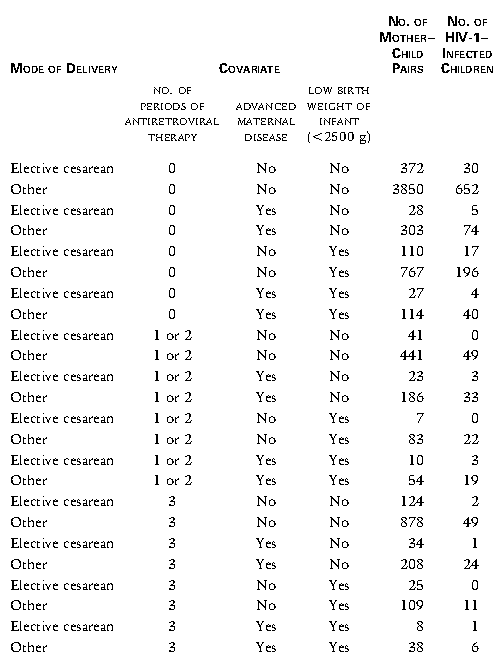
\includegraphics[scale=1.1]{~/git_repositories/epib607/inst/slides/024-logistic-reg-1/hivtable.pdf}
\end{figure}




\begin{table}[H]
	\centering
	\begin{tabular}{lcc|c}
		& Exposed  &   Unexposed & Total  \\		
		Cases    & $a_i$ &  $b_i$ & $M_{1i}$ \\
		Controls & $c_i$ 	& $d_i$  	& $M_{0i}$ 	\\	
		\hline
		Total & $N_{1i}$ & $N_{0i}$ 	& $T_i$
	\end{tabular}
\end{table}


$OR_{MH} = \frac{\sum_i \frac{a_i d_i}{T_i}}{\sum_i \frac{b_i c_i}{T_i}}$ \\ \ \\
$RR_{MH} = \frac{\sum_i \frac{a_i N_{0i}}{T_i}}{\sum_i \frac{b_i N_{1i}}{T_i}}$

\end{frame}




\begin{frame}[fragile,plain]
	\vspace{-.81in}
	\tiny
\begin{knitrout}\small
\definecolor{shadecolor}{rgb}{0.969, 0.969, 0.969}\color{fgcolor}\begin{kframe}
\begin{verbatim}
## Call:
## glm(formula = cbind(n.hivpos, n.hivneg) ~ 1, family = binomial(link = logit), 
##     data = ds)
## 
## Coefficients:
##             Estimate Std. Error z value Pr(>|z|)    
## (Intercept)   -1.671      0.031     -54   <2e-16 ***
## ---
## Signif. codes:  0 '***' 0.001 '**' 0.01 '*' 0.05 '.' 0.1 ' ' 1
## 
## (Dispersion parameter for binomial family taken to be 1)
## 
##     Null deviance: 293.95  on 23  degrees of freedom
## Residual deviance: 293.95  on 23  degrees of freedom
## AIC: 387.8
## 
## Number of Fisher Scoring iterations: 4
\end{verbatim}
\end{kframe}
\end{knitrout}


\begin{knitrout}\small
\definecolor{shadecolor}{rgb}{0.969, 0.969, 0.969}\color{fgcolor}\begin{kframe}
\begin{verbatim}
## Call:
## glm(formula = cbind(n.hivpos, n.hivneg) ~ caesarian, family = binomial(link = logit), 
##     data = ds)
## 
## Coefficients:
##             Estimate Std. Error z value Pr(>|z|)    
## (Intercept)   -1.606      0.032   -50.2   <2e-16 ***
## caesarian     -0.815      0.132    -6.2    7e-10 ***
## ---
## Signif. codes:  0 '***' 0.001 '**' 0.01 '*' 0.05 '.' 0.1 ' ' 1
## 
## (Dispersion parameter for binomial family taken to be 1)
## 
##     Null deviance: 293.95  on 23  degrees of freedom
## Residual deviance: 247.78  on 22  degrees of freedom
## AIC: 343.7
## 
## Number of Fisher Scoring iterations: 4
\end{verbatim}
\end{kframe}
\end{knitrout}

\end{frame}

\vspace{-0.3in}

\begin{knitrout}\small
\definecolor{shadecolor}{rgb}{0.969, 0.969, 0.969}\color{fgcolor}\begin{kframe}
\begin{verbatim}
## Call:
## glm(formula = cbind(n.hivpos, ds$n.hivneg) ~ caesarian + ART1or2 + 
##     ART3 + m.advancedHIV + c.LBW, family = binomial(link = logit), 
##     data = ds)
## 
## Coefficients:
##               Estimate Std. Error z value Pr(>|z|)    
## (Intercept)     -1.608      0.041   -39.6   <2e-16 ***
## caesarian       -0.852      0.134    -6.3    2e-10 ***
## ART1or2         -0.362      0.106    -3.4    6e-04 ***
## ART3            -1.178      0.114   -10.3   <2e-16 ***
## m.advancedHIV    0.535      0.090     6.0    3e-09 ***
## c.LBW            0.581      0.075     7.8    9e-15 ***
## ---
## Signif. codes:  0 '***' 0.001 '**' 0.01 '*' 0.05 '.' 0.1 ' ' 1
## 
## (Dispersion parameter for binomial family taken to be 1)
## 
##     Null deviance: 293.945  on 23  degrees of freedom
## Residual deviance:  18.393  on 18  degrees of freedom
## AIC: 122.3
## 
## Number of Fisher Scoring iterations: 4
\end{verbatim}
\end{kframe}
\end{knitrout}

\vspace{-0.22in}

\begin{knitrout}\small
\definecolor{shadecolor}{rgb}{0.969, 0.969, 0.969}\color{fgcolor}\begin{kframe}
\begin{verbatim}
## Call:
## glm(formula = cbind(n.hivpos, ds$n.hivneg) ~ caesarian + ART1or2 + 
##     ART3 + m.advancedHIV + c.LBW, family = binomial(link = log), 
##     data = ds)
## 
## Coefficients:
##               Estimate Std. Error z value Pr(>|z|)    
## (Intercept)     -1.793      0.034   -53.2   <2e-16 ***
## caesarian       -0.720      0.119    -6.0    2e-09 ***
## ART1or2         -0.278      0.087    -3.2    0.001 ** 
## ART3            -1.016      0.104    -9.8   <2e-16 ***
## m.advancedHIV    0.409      0.068     6.0    2e-09 ***
## c.LBW            0.453      0.057     7.9    2e-15 ***
## ---
## Signif. codes:  0 '***' 0.001 '**' 0.01 '*' 0.05 '.' 0.1 ' ' 1
## 
## (Dispersion parameter for binomial family taken to be 1)
## 
##     Null deviance: 293.945  on 23  degrees of freedom
## Residual deviance:  21.295  on 18  degrees of freedom
## AIC: 125.2
## 
## Number of Fisher Scoring iterations: 5
\end{verbatim}
\end{kframe}
\end{knitrout}




\section{Smoking among women in Whickham, UK}



Consider the following \textit{age stratified} mortality data (Rothman, Table 1-2) from a study that looked at smoking habits of residents of Whickham, England, in the period 1972-1974 and then tracked the survival over the next 20 years of those who were interviewed. 


\begin{table}[h]
	\centering
	\begin{tabular}{lcccc}
		&  &   \multicolumn{2}{c}{Smoking} &  \\		
		Age & Vital Status &  Yes & No & Total \\
		18-24 	& Dead 	& 2  	& 1 	& 3 	\\	
		& Alive & 53  	& 61 	& 114 	\\
		& Risk & 0.04  	& 0.02 	& 0.03 	\\
		\hline
		25-34 	& Dead 	& 3  	& 5 	& 8 	\\	
		& Alive & 121  	& 152 	& 273 	\\
		& Risk & 0.02  	& 0.03 	& 0.03 \\
		\hline 			
		35-44 	& Dead 	& 14  	& 7 	& 21 	\\	
		& Alive & 95  	& 114 	& 209 	\\
		& Risk & 0.13  	& 0.06 	& 0.09 \\
		\hline
		45-54 	& Dead 	& 27  	& 12 	& 39 	\\	
		& Alive & 103  	& 66 	& 169 	\\
		& Risk & 0.21  	& 0.15 	& 0.19 \\
		\hline
		55-64 	& Dead 	& 51  	& 40 	& 91 	\\	
		& Alive & 64  	& 81 	& 145 	\\
		& Risk & 0.44  	& 0.33 	& 0.39 \\
		\hline
		65-74 	& Dead 	& 29  	& 101 	& 130 	\\	
		& Alive & 7  	& 28 	& 35 	\\
		& Risk & 0.81  	& 0.78 	& 0.79 \\
		\hline
		75+ 	& Dead 	& 13  	& 64 	& 77 	\\	
		& Alive & 0  	& 0 	& 0 	\\
		& Risk & 1.00  	& 1.00 	& 1.00 \\
		\hline
	\end{tabular}
\end{table}



\begin{frame}[fragile]{Session Info}
	\tiny
	
\begin{knitrout}\tiny
\definecolor{shadecolor}{rgb}{0.969, 0.969, 0.969}\color{fgcolor}\begin{kframe}
\begin{verbatim}
R version 4.1.1 (2021-08-10)
Platform: x86_64-pc-linux-gnu (64-bit)
Running under: Pop!_OS 21.04

Matrix products: default
BLAS:   /usr/lib/x86_64-linux-gnu/openblas-pthread/libblas.so.3
LAPACK: /usr/lib/x86_64-linux-gnu/openblas-pthread/libopenblasp-r0.3.13.so

attached base packages:
[1] tools     stats     graphics  grDevices utils     datasets  methods  
[8] base     

other attached packages:
 [1] DT_0.16           mosaic_1.7.0      Matrix_1.3-2      mosaicData_0.20.1
 [5] ggformula_0.9.4   ggstance_0.3.4    lattice_0.20-41   kableExtra_1.2.1 
 [9] socviz_1.2        gapminder_0.3.0   here_0.1          NCStats_0.4.7    
[13] FSA_0.8.30        forcats_0.5.1     stringr_1.4.0     dplyr_1.0.7      
[17] purrr_0.3.4       readr_1.4.0       tidyr_1.1.4       tibble_3.1.5     
[21] ggplot2_3.3.5     tidyverse_1.3.0   knitr_1.36       

loaded via a namespace (and not attached):
 [1] fs_1.5.0           lubridate_1.7.9    webshot_0.5.2      httr_1.4.2        
 [5] rprojroot_2.0.2    backports_1.2.1    utf8_1.2.2         R6_2.5.1          
 [9] DBI_1.1.1          colorspace_2.0-2   withr_2.4.2        tidyselect_1.1.1  
[13] gridExtra_2.3      leaflet_2.0.3      curl_4.3.2         compiler_4.1.1    
[17] cli_3.0.1          rvest_1.0.0        pacman_0.5.1       xml2_1.3.2        
[21] ggdendro_0.1.22    mosaicCore_0.8.0   scales_1.1.1       digest_0.6.28     
[25] foreign_0.8-81     rmarkdown_2.11.3   rio_0.5.16         pkgconfig_2.0.3   
[29] htmltools_0.5.2    highr_0.9          dbplyr_1.4.4       fastmap_1.1.0     
[33] htmlwidgets_1.5.3  rlang_0.4.12       readxl_1.3.1       rstudioapi_0.13   
[37] farver_2.1.0       generics_0.1.0     jsonlite_1.7.2     crosstalk_1.1.1   
[41] zip_2.2.0          car_3.0-9          magrittr_2.0.1     Rcpp_1.0.7        
[45] munsell_0.5.0      fansi_0.5.0        abind_1.4-5        lifecycle_1.0.1   
[49] stringi_1.7.5      carData_3.0-4      MASS_7.3-53.1      plyr_1.8.6        
[53] grid_4.1.1         blob_1.2.1         ggrepel_0.8.2      crayon_1.4.1      
[57] cowplot_1.1.0      haven_2.3.1        splines_4.1.1      hms_1.1.1         
[61] pillar_1.6.4       reprex_0.3.0       glue_1.4.2         evaluate_0.14     
[65] data.table_1.14.2  modelr_0.1.8       vctrs_0.3.8        tweenr_1.0.1      
[69] cellranger_1.1.0   gtable_0.3.0       polyclip_1.10-0    assertthat_0.2.1  
[73] TeachingDemos_2.12 xfun_0.26          ggforce_0.3.2      openxlsx_4.1.5    
[77] broom_0.7.9        viridisLite_0.4.0  ellipsis_0.3.2    
\end{verbatim}
\end{kframe}
\end{knitrout}
	
\end{frame}


\end{document}
